%%%%%%%%%%%%%%%%%%%%%%%%%%%%%%%%%%%%%%%%%
% Cheatsheet
% LaTeX Template
% Version 1.0 (12/12/15)
%
% This template has been downloaded from:
% http://www.LaTeXTemplates.com
%
% Original author:
% Michael Müller (https://github.com/cmichi/latex-template-collection) with
% extensive modifications by Vel (vel@LaTeXTemplates.com)
%
% License:
% The MIT License (see included LICENSE file)
%
%%%%%%%%%%%%%%%%%%%%%%%%%%%%%%%%%%%%%%%%%

%----------------------------------------------------------------------------------------
%	PACKAGES AND OTHER DOCUMENT CONFIGURATIONS
%----------------------------------------------------------------------------------------

\documentclass[11pt]{scrartcl} % 11pt font size

\usepackage[utf8]{inputenc} % Required for inputting international characters
\usepackage[T1]{fontenc} % Output font encoding for international characters

\usepackage{tikz}

\usepackage[margin=0pt, landscape]{geometry} % Page margins and orientation

\usepackage{graphicx} % Required for including images

\usepackage{color} % Required for color customization
\definecolor{mygray}{gray}{.75} % Custom color

\usepackage{url} % Required for the \url command to easily display URLs

\usepackage[ % This block contains information used to annotate the PDF
colorlinks=false, 
pdftitle={Cheatsheet}, 
pdfauthor={John Smith}, 
pdfsubject={Compilation of useful shortcuts}, 
pdfkeywords={Random Software, Cheatsheet}
]{hyperref}

\setlength{\unitlength}{1mm} % Set the length that numerical units are measured in
\setlength{\parindent}{0pt} % Stop paragraph indentation

\renewcommand{\dots}{\ \dotfill{}\ } % Fills in the right amount of dots

\newcommand{\command}[2]{#1~\dotfill{}~#2\\} % Custom command for adding a shorcut

\newcommand{\sectiontitle}[1]{\textbf{#1}} % Custom command for subsection titles

%----------------------------------------------------------------------------------------

\begin{document}

\begin{picture}(297,210) % Create a container for the page content

%----------------------------------------------------------------------------------------
%	TITLE SECTION 
%----------------------------------------------------------------------------------------

%\put(10,200){ % Position on the page to put the title
%\begin{minipage}[t]{210mm} % The size and alignment of the title
%\section*{Cheatsheet Template -- Application Shortcuts} % Title
%\end{minipage}
%}

%----------------------------------------------------------------------------------------
%	FIRST COLUMN SPECIFICATION
%----------------------------------------------------------------------------------------

\put(1,205){ % Divide the page
\begin{minipage}[t]{96.33mm} % Create a box to house text

%----------------------------------------------------------------------------------------
%	HEADING ONE
%----------------------------------------------------------------------------------------

\sectiontitle{Discrete system recap}

Euler Discretization: $x(k+1) = x(k) + T_sg^c(x(k),u(k))$
Euler model -> DT: $A = I + T_s A^c, B = T_sB^c$ \\
Exact Discretization: $A = e^{A^c T_s}, B = (A^c)^{-1}(A-I)B^c$
Solution: $x(k+N) = A^Nx(k) + \sum_{i=0}^{N-1} A^iBu(k+N-1-i)$
Taylor of exponential: $e^{A^c T_s} = \sum_{n=0}^{\infty}\frac{(A^ct)^n}{n!}$

\sectiontitle{Coordinate Transformation}

considering: $\tilde{x}(k) = Tx(k)$, then $\tilde{A} = TAT^{-1}, \tilde{B} = TB, \tilde{C} = CT^{-1}, \tilde{D} = D$

\sectiontitle{Stability, Controlability, Observability (Linear)}

Stable iff: $|\lambda_j| < 1$, where $\lambda$ eigenvlaues of A \\
Controllability (nec and suff): rank([$B AB ... A^{n-1}B$]) = $n$\\
Obs (nec and suff): rank([$C^T (CA)^T ... (CA^{n-1})^T$]$^T$) = $n$

\sectiontitle{Lyapunov Stability non-linear}

system of form: $x(k+1) = g(x(k))$, with \emph{equilibrium point} at $\bar{x}$, i.e. $g(\bar{x}) = \bar{x}$.
Find a lyapunov function $V(x)$ that satisfies the following constraints: $V(0) = 0 \textit{ and } V(x) > 0, \forall x \in \Omega$. 
$V(g(x)) - V(x) \leq -\alpha(x) \forall x \in \Omega$\\
If a V(x) is admitted then x = 0 is \textbf{asymptotically stable}. If, however, $\alpha(x)$ is positive semi-definite, it is Lyapunov stable in $\Omega$. If additionally, V goes to infinity as x goes to infinity, x = 0 is globally asymptotically stable.\\
\textbf{Indirect method}

Linearize to obtain A matrix. If all ev's stable, then the origin is asymptotically stable. If one ev is not stable, then the origin is unstable. If at least 1 ev is on the border, no conclusions can be drawn.

\textbf{Global Lyapunov stability of Linear Systems}

System: $x(k+1) = Ax(k)$, Lyapunov fct: $V(x) = x^TPx$, $P>0$. Energy decresase condition: $V(Ax(k)) - V(x(k)) = x^T(k)(A^TPA-P)x(k) \leq -\alpha(x(k))$. Choose $\alpha(x(k)) = x^T(k)Qx(k), Q > 0$. $\Rightarrow$ find $P>0$ with $A^TPA-P = -Q, Q>0$. Theorem: unique solution $P>0$ exists, iff $|\lambda_i (A)| < 1$. Stability is always global for linear systems.



\begin{tikzpicture}
\begin{scope}[xshift=1.5cm]
    \node[anchor=south west,inner sep=0] (image) at (0,0) {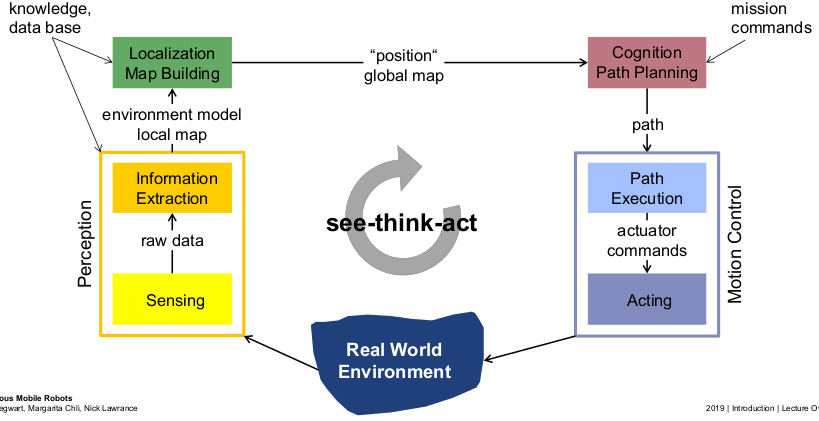
\includegraphics[width=0.7\textwidth]{figures/latexTemplate.png}};
    
    \begin{scope}[x={(image.south east)},y={(image.north west)}]
    	\node [anchor=west] (test) at (1.1,0.7) {test};
        \draw[red,ultra thick,rounded corners] (0.44,0.80) rectangle (0.55,0.95);
        \draw [-latex, ultra thick, red] (test.west) to[out=-180, in=-120] (0.48,0.80);
    \end{scope}
    
\end{scope}
\end{tikzpicture}%

%----------------------------------------------------------------------------------------

\end{minipage} % End the first column of text
} % End the first division of the page

%----------------------------------------------------------------------------------------
%	SECOND COLUMN SPECIFICATION 
%----------------------------------------------------------------------------------------

\put(100.33,205){ % Divide the page
\begin{minipage}[t]{96.33mm} % Create a box to house text

%----------------------------------------------------------------------------------------
%	HEADING FOUR
%----------------------------------------------------------------------------------------

\sectiontitle{Navigation}

\command{Mod4 + j}{Focus next client}
\command{Mod4 + k}{Focus previous client}
\command{Mod4 + u}{Focus first urgent client}
\command{Mod4 + Left}{View previous tag}
\command{Mod4 + Right}{View next tag}
\command{Mod4 + 1-9}{Switch to tag 1-9}
\command{Mod4 + Ctrl + j}{Focus next screen}
\command{Mod4 + Ctrl + k}{Focus previous screen}
\command{Mod4 + j}{Focus next client}
\command{Mod4 + k}{Focus previous client}
\command{Mod4 + u}{Focus first urgent client}
\command{Mod4 + Esc}{Focus previously selected tag set}
					
%----------------------------------------------------------------------------------------
%	HEADING FIVE
%----------------------------------------------------------------------------------------				
					
\sectiontitle{Layout modification} % Heading five

\command{Mod4 + Shift + k / j}{Rotate clients around}
\command{Mod4 + h / l}{Change master width by 5\%}
\command{Mod4 + Shift + h}{Number of master windows +1}
\command{Mod4 + Shift + l}{Number of master windows --1}
\command{Mod4 + Ctrl + h}{Number of columns for non-master windows +1}
\command{Mod4 + Ctrl + l}{Number of columns for non-master windows --1}

\command{Mod4 + Space}{Next layout}
\command{Mod4 + Shift + Space}{Previous layout}
\command{Mod4 + Ctrl + Space}{Floating master}
\command{Mod4 + Ctrl + Return}{Swap focused client with master}

%----------------------------------------------------------------------------------------


		

\end{minipage} % End the second column of text
} % End the second division of the page

%----------------------------------------------------------------------------------------
%	THIRD COLUMN SPECIFICATION 
%----------------------------------------------------------------------------------------

\put(199.66,180){ % Divide the page
\begin{minipage}[t]{96.33mm} % Create a box to house tex

%----------------------------------------------------------------------------------------
%	IMPORTANT FILES
%----------------------------------------------------------------------------------------

\sectiontitle{Important files}

\texttt{/.config/awesome/rc.lua}

\texttt{/etc/xdg/awesome/rc.lua}

\vspace{\baselineskip} % Whitespace before the next section

%----------------------------------------------------------------------------------------
%	LINKS AND INFORMATION
%----------------------------------------------------------------------------------------

\sectiontitle{Links and information}

\url{http://awesome.naquadah.org/}

\url{http://awesome.naquadah.org/wiki/}

%----------------------------------------------------------------------------------------
%	FOOTNOTE
%----------------------------------------------------------------------------------------

\vspace{\baselineskip}
\linethickness{0.5mm} % Thickness of the footer line
{\color{mygray}\line(1,0){30}} % Print the line with a custom color

\footnotesize{
Created by John Smith, 2015\\ 
\url{http://johnsmith.com/}\\
				
Released under the MIT license.
}

%----------------------------------------------------------------------------------------

\end{minipage} % End the third column of text
} % End the third division of the page
\end{picture} % End the container for the entire page

%----------------------------------------------------------------------------------------

\end{document}